%!TEX root = ../Thesis.tex

\chapter{Evaluation and optimization}
	During the course of creating the application we tried different approaches to several interim steps. In this chapter we discuss how using different algorithms yielded different results.

	\section{Dataset}
	In order to test and optimize our detector we created a set of 101 images and annotated them manually with the following information: each intersection on the board was marked with a point, either as an empty intersection, an intersection with a white piece on it or one occupied by a black piece. Also, the location of all pieces was marked with a circle, i.e. with a center and its approximate radius.

	To have an image set that covers as many possible game situations as possible we took pictures in three different lighting conditions and on different backgrounds. Each time we took images of an empty board without any pieces, a board with only some few images and a configuration as it often happens during endgame. That is, many pieces on the board and lots of them in a line.

	Each board configuration was photographed from different angles in $\varphi$ (azimuth) and $\theta$ (polar) direction and from two directions, i.e. facing the board from the side a player would and rotated by 90\textdegree~ as a third person would see the board.

	\begin{figure}
		\begin{subfigure}[b]{0.3\textwidth}
			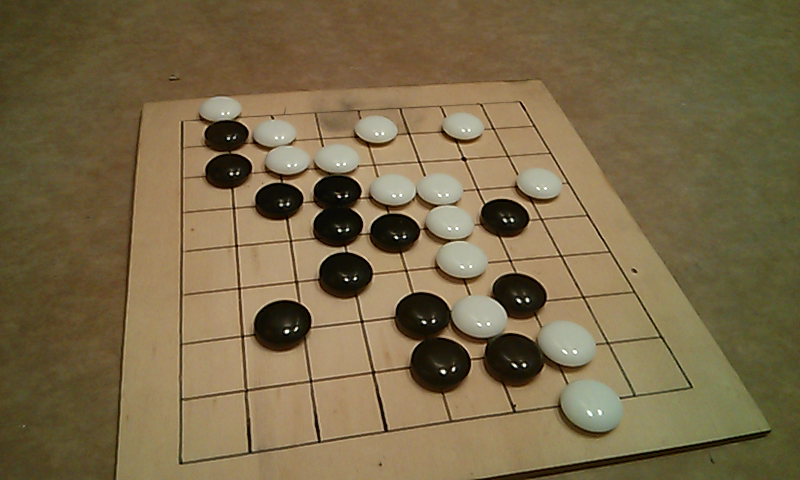
\includegraphics[width=\textwidth]{images/warmLight_many_leftMedium.png}
			\caption{Paper in warm light; camera left on medium height}
		\end{subfigure}
		~
		\begin{subfigure}[b]{0.3\textwidth}
				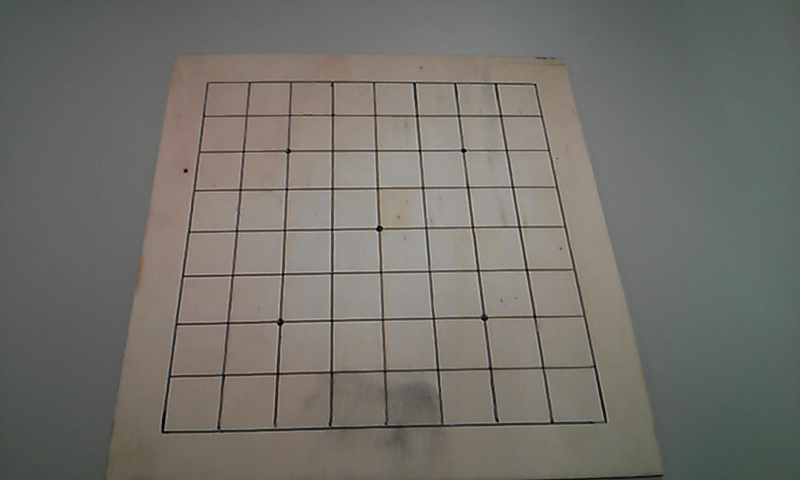
\includegraphics[width=\textwidth]{images/neonDesk_empty_centerAbove.png}
				\caption{Plain gray desk in neon light; camera centered high}
		\end{subfigure}
		~
		\begin{subfigure}[b]{0.3\textwidth}
				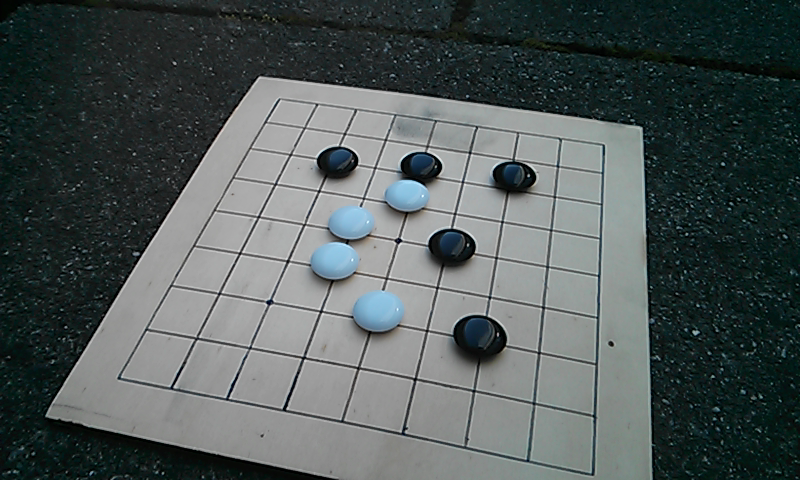
\includegraphics[width=\textwidth]{images/shadowStone_some_rightAbove.png}
				\caption{Dark stone surface in the shadow; camera right high}
		\end{subfigure}
		\\
		\begin{subfigure}[b]{0.3\textwidth}
				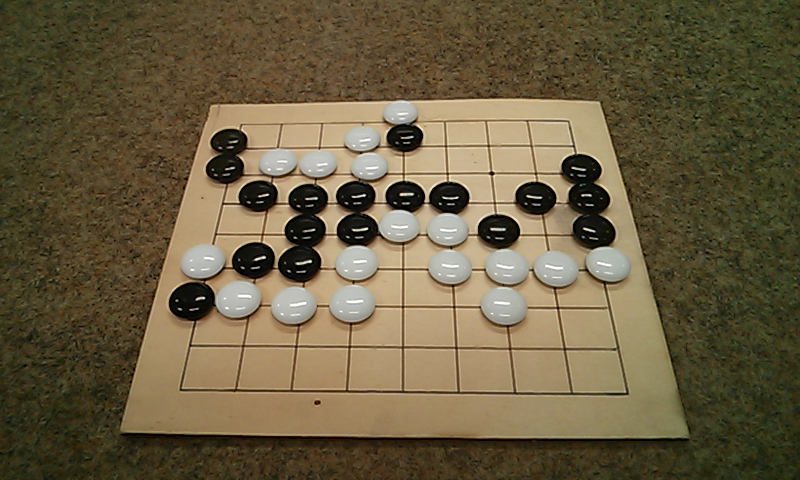
\includegraphics[width=\textwidth]{images/neonFloor_many_centerLow.png}
				\caption{Brown carpet in neon light; camera centered low}
		\end{subfigure}
		~
		\begin{subfigure}[b]{0.3\textwidth}
				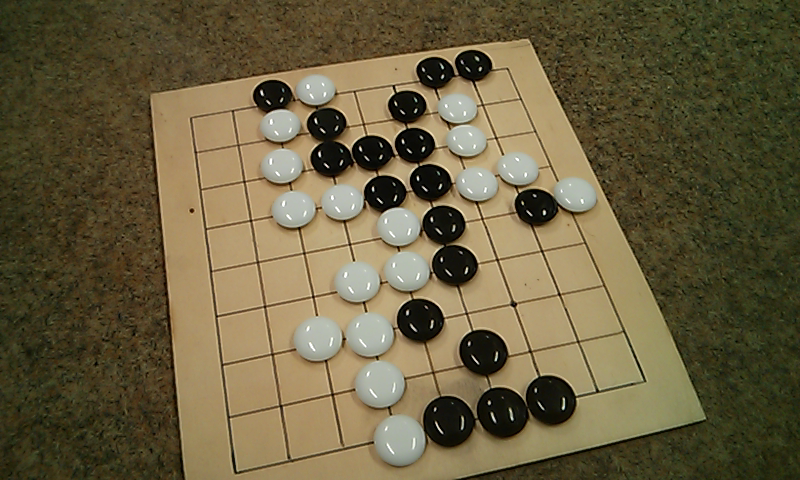
\includegraphics[width=\textwidth]{images/neonFloor_many_centerLow_rotated.png}
				\caption{Like (d) but from bystanders'	 perspective}
		\end{subfigure}
		~
		\begin{subfigure}[b]{0.3\textwidth}
			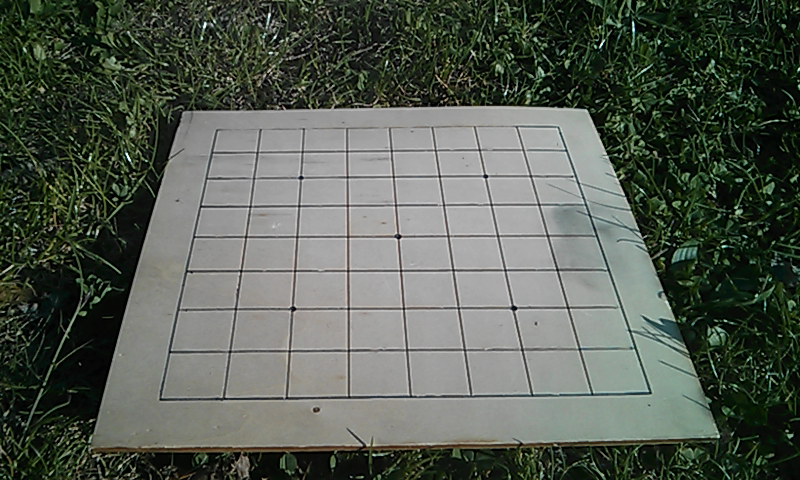
\includegraphics[width=\textwidth]{images/sunnyGrass_empty_centerLow.png}
			\caption{On grass in sunlight; camera centered low}
		\end{subfigure}

		\caption{Some examples of different lighting conditions, angles and backgrounds as well as different piece count}
		\label{fig:sampeImages}
	\end{figure}

	We ended up with: 29 images taken in cold neon light on a plain gray desk; 26 images taken in the same light on a textured, brown carpet; 25 images taken on a sunny day in the shadow on a stone surface; 17 images in warm artificial light on a textured paper background. Furthermore we have 5 images taken in the sun on an evening in which the board lay in grass. See \ref{fig:sampeImages} for some examples from the image set.

	The images were taken by starting the app normally but then instead of starting detection saving the input image on the internal memory of the device. While in the beginning we saved images to png we later switched to persisting the images into yml format and retake the previous images. This has the advantage that we can be absolutely sure that the input to our test instances are the same as they would be on a phone, as no png coding and decoding takes place. Also we had problems in the beginning because OpenCV's image persisting function presumably does not recognize that the camera image is encoded in RGB (see \ref{android-detector}), which lead to different results on our desktop hardware than on our Android phone.

	31 of the images were randomly chosen as a test set evenly spread over all lighting conditions as well as piece and angle configurations. The grass images were not part of the test set as they soon turned out to be very difficult. We included them in the training set, though. This set was used to improve our detector.

	To do so we assumed that there is a global maximum for the overall quality of results when adjusting parameters of the used algorithms. Even if this assumption were wrong we optimized for a local maximum. Then we tried manually to find roughly the optimal parameters for some randomly chosen images for every algorithm. Finally we adjusted them automatedly by brute forcely trying every combination of parameters in the vicinity of the manually chosen on every image on a cluster of 45 oktacore machines and checking the results against the annotations.

	\section{Visible intersections}
	%TODO: eigentlich ist visible intersections falsch, weil ja auch unsichtbare gematcht werden
	When evaluating the detection rate of visible intersections we first checked if the intersection was within the boundaries of the annotated board and a padding of 15 pixels. If not the intersection was considered uninteresting and did neither count positively nor negatively. If it was inside the board we searched the nearest annotated intersection for every detected one. If there was none within a range of 15 pixels the intersection was counted as a false positive. But if there was, then the annotated intersection was marked as detected and not considered as a possible match for other intersections. The threshold was chosen roughly as a quarter of the average distance between two intersections and a third of the diameter of a piece as measured in some sample images.

	%!TEX root = ../Thesis.tex

\begin{figure}
	\pgfplotsset{width=\textwidth, height=5.5cm, compat=1.11}
	\begin{subfigure}{\textwidth}
		\begin{tikzpicture}
			\begin{semilogyaxis}[
				ylabel={Intersections count},
				xlabel={Different parameter combinations},
				xtick style={draw=none},
				xticklabels={,,},
				axis x line=bottom,
				axis y line=left,
				legend style={at={(1,0.05)}, anchor=south east},
				xmin=0,
				ymin=0,
				xmax=610,
				ymax=6000
				]
				\draw[white!70!black, thin] ({rel axis cs:1,0}|-{axis cs:0,5670}) -- ({rel axis cs:0,0}|-{axis cs:0,5670});
				\draw[white!70!black, thin] ({rel axis cs:1,0}|-{axis cs:0,70}) -- ({rel axis cs:0,0}|-{axis cs:0,70});
				\draw[orange, thick] ({axis cs:381,5000}) -- ({axis cs:381,0}|-{rel axis cs:0,0});
				\draw[orange, thick] ({axis cs:0,5000}) -- ({axis cs:381,5000});

				\addplot[color=red, smooth]          table[x expr=\coordindex+1, y=matched, mark=none] {plots/lines_hough_part.csv};
				\addplot[color=red!40!black, smooth] table[x expr=\coordindex+1, y=wrong, mark=none] {plots/lines_hough_part.csv};

				\addlegendentry{Sum of true positives on all images}
				\addlegendentry{Sum of all false positives on all images}
			\end{semilogyaxis}
		\end{tikzpicture}
		\vspace{-20pt}
		\caption{Representative subset of 605 combinations of 60481 tested for the Houghline detector}
		\label{fig:linesTraining-hough}
	\end{subfigure}
	\vspace{20pt}

	\begin{subfigure}{\textwidth}
		\begin{tikzpicture}
			\begin{semilogyaxis}[
				ylabel={Intersections count},
				xlabel={Different parameter combinations},
				xtick style={draw=none},
				xticklabels={,,},
				axis x line=bottom,
				axis y line=left,
				legend style={at={(1,0.05)}, anchor=south east},
				xmin=0,
				ymin=0,
				xmax=610,
				ymax=6000
				]
				\draw[white!70!black, thin] ({rel axis cs:1,0}|-{axis cs:0,5670}) -- ({rel axis cs:0,0}|-{axis cs:0,5670});
				\draw[white!70!black, thin] ({rel axis cs:1,0}|-{axis cs:0,70}) -- ({rel axis cs:0,0}|-{axis cs:0,70});
				\draw[orange, thick] ({axis cs:158,1175}) -- ({axis cs:158,0}|-{rel axis cs:0,0});
				\draw[orange, thick] ({axis cs:0,1175}) -- ({axis cs:158,1175});

				\addplot[color=blue, smooth]          table[x expr=\coordindex+1, y=matched, mark=none, smooth,] {plots/lines_lsd_part.csv};
				\addplot[color=blue!40!black, smooth] table[x expr=\coordindex+1, y=wrong, mark=none, smooth, blue] {plots/lines_lsd_part.csv};

				\addlegendentry{Sum of true positives on all images}
				\addlegendentry{Sum of all false positives on all images}
			\end{semilogyaxis}
		\end{tikzpicture}
		\vspace{-20pt}
		\caption{Representative subset of 605 combinations of 58321 tested for the LSD detector.}
		\label{fig:linesTraining-lsd}
	\end{subfigure}
	\vspace{20pt}

	\begin{subfigure}{\textwidth}
		\begin{tikzpicture}
			\begin{semilogyaxis}[
				ylabel={Intersections count},
				xlabel={Different parameter combinations},
				xtick style={draw=none},
				xticklabels={,,},
				axis x line=bottom,
				axis y line=left,
				legend style={at={(1,0.05)}, anchor=south east},
				xmin=0,
				ymin=0,
				xmax=610,
				ymax=15000
				]
				\draw[white!70!black, thin] ({rel axis cs:1,0}|-{axis cs:0,5670}) -- ({rel axis cs:0,0}|-{axis cs:0,5670});
				\draw[white!70!black, thin] ({rel axis cs:1,0}|-{axis cs:0,70}) -- ({rel axis cs:0,0}|-{axis cs:0,70});
				\draw[orange, thick] ({axis cs:117,215}) -- ({axis cs:117,0}|-{rel axis cs:0,0});
				\draw[orange, thick] ({axis cs:0,215}) -- ({axis cs:117,215});

				\addplot[color=green, smooth]          table[x expr=\coordindex+1, y=matched, mark=none, smooth,] {plots/intersects_fast_part.csv};
				\addplot[color=green!40!black, smooth] table[x expr=\coordindex+1, y=wrong, mark=none, smooth, blue] {plots/intersects_fast_part.csv};

				\addlegendentry{Sum of true positives on all images}
				\addlegendentry{Sum of all false positives on all images}
			\end{semilogyaxis}
		\end{tikzpicture}
		\vspace{-20pt}
		\caption{Representative subset of 605 combinations of 1440 tested for the FAST detector}
		\label{fig:linesTraining-fast}
	\end{subfigure}

	\caption{The x-axis shows different combinations of parameters that we have evaluated. On the y-axis the true positives, false positives, totally available intersections (upper gray line) and number of analyzed images (lower gray line) per combination can be seen. The x-axis does not imply any order of the tested combinations; results have been simply sorted after number of correct intersections. We chose the parameter combination with the highest true positive rate whilst less false positives than evaluated files (orange line)}
	\label{fig:linesTraining}
\end{figure}


	\subsection{Optimizations on the training set}
	While optimizing the parameters used in our algorithm, we measured the quality as the ratio of detected to undetected intersections, also considering the number of false positives. Traditionally one would calculate some ratio of true positives to false positives. However none of the usual measurement methods shows us a clear indicator what combinations of parameters to use, so we devised the following metric: We sorted the results by the number of correctly matched intersections and chose the highest one where the number of false positives was lower or equal than the number of images recognized ($|false\_positives| \leq |input\_images|$, i.e. statistically maximal one false positive per image). This is shown (albeit on a representative subset of all tested parameter combinations) in \ref{optimizationlinesCorrectness}, where the parameters we chose is marked in orange.

	\subsubsection{HOUGH}
	In comparison to the other algorithms detecting the lines using Hough transformation performs best quality-wise. As \ref{fig:houghCorrectness} shows, we still had to compromise when choosing the final parameter set. The one we chose as noted above resulted in 89.67\% (5084 out of 5670) correct detection rate in our training set, with a total of 68 incorrect intersections (0.01199\% of available intersections).

	The graphic shows also that that the quality of the line detection does not depend very much on the parameters used: there's only a few parameter combinations that yield very poor results and hardly any that results in finding no intersection at all. As would be expected the average number of false positives rises with the percentage of correctly found intersections. Luckily, there is enough variance yet that even at a high detection rate we can find entries with on average less than one false intersection per image.

	\subsubsection{LSD}
	As noted in \ref{detector-visible-lsd} the Line Segment Detector needs significant postprocessing to give any reasonable results. Still it is easily outperformed by the variant using hough transformation. In \ref{fig:lsdCorrectness} it can easily be seen that the amount of false positives does not go below the amount of input images when roughly a quarter of all available intersections should be detected. Furthermore the average ratio of correct results to false positives is nearly over all combinations worse than its hough counterpart's. Only in the segment where both detect nearly 100\% of all correct intersections. The total number of wrong intersections ranges in the thousands here, though, making this segment unusable for the application.

	\subsubsection{FAST}
	Even worse performs the FAST corner detector when used for detection of the intersections. It is the only detector that resulted in more false positives than correct intersections in some combination. The ratio of false positives to correct intersections is in no combination better than the of the intersections of lines detected using LSD or Hough transformation.

	\subsection{Performance on the testing set}

	%!TEX root = ../Thesis.tex

\begin{figure}
	\pgfplotsset{width=\textwidth, height=5cm, compat=1.11}
	\begin{subfigure}{0.32\textwidth}
		\begin{tikzpicture}
			\begin{axis}[
				xticklabels={,,},
				axis x line=bottom,
				axis y line=left,
				xmin=0,
				ymin=0,
				xmax=32,
				ymax=1
				]
				\draw[gray] ({rel axis cs:1,0}|-{axis cs:0,81}) -- ({rel axis cs:0,0}|-{axis cs:0,81});

				\addplot[only marks, mark=*, mark options={scale=1.1, fill=red!40!black}]
					table[x expr=\coordindex+1, y expr=\thisrow{matched}/(\thisrow{matched}+\thisrow{wrong})] {plots/lines_hough_testSet.csv};
				\addplot[only marks, mark=*, mark options={scale=1.1, fill=red}]
					table[x expr=\coordindex+1, y expr=\thisrow{matched}/81] {plots/lines_hough_testSet.csv};
			\end{axis}
		\end{tikzpicture}
		\caption{Results of the Hough transformation detector}
		\label{fig:linesTest-hough}
	\end{subfigure}
	\hfill
	\begin{subfigure}{0.32\textwidth}
		\begin{tikzpicture}
			\begin{axis}[
				xticklabels={,,},
				axis x line=bottom,
				axis y line=left,
				xmin=0,
				ymin=0,
				xmax=32,
				ymax=1
				]
				\draw[gray] ({rel axis cs:1,0}|-{axis cs:0,81}) -- ({rel axis cs:0,0}|-{axis cs:0,81});

				\addplot[only marks, mark=*, mark options={scale=1.1, fill=blue!40!black}]
					table[x expr=\coordindex+1, y expr=\thisrow{matched}/(\thisrow{matched}+\thisrow{wrong})] {plots/lines_lsd_testSet.csv};
				\addplot[only marks, mark=*, mark options={scale=1.1, fill=blue}]
					table[x expr=\coordindex+1, y expr=\thisrow{matched}/81] {plots/lines_lsd_testSet.csv};
			\end{axis}
		\end{tikzpicture}
		\caption{Results of the LSD detector}
		\label{fig:linesTest-lsd}
	\end{subfigure}
	\hfill
	\begin{subfigure}{0.32\textwidth}
		\begin{tikzpicture}
			\begin{axis}[
				xticklabels={,,},
				axis x line=bottom,
				axis y line=left,
				xmin=0,
				ymin=0,
				xmax=32,
				ymax=1
				]
				\draw[gray] ({rel axis cs:1,0}|-{axis cs:0,81}) -- ({rel axis cs:0,0}|-{axis cs:0,81});

				\addplot[only marks, mark=*, mark options={scale=1.1, fill=green!40!black}]
					table[x expr=\coordindex+1, y expr=\thisrow{matched}/(\thisrow{matched}+\thisrow{wrong})] {plots/intersections_fast_testSet.csv};
				\addplot[only marks, mark=*, mark options={scale=1.1, fill=green}]
					table[x expr=\coordindex+1, y expr=\thisrow{matched}/81] {plots/intersections_fast_testSet.csv};
			\end{axis}
		\end{tikzpicture}
		\caption{Results of the corner detector}
		\label{fig:linesTest-fast}
	\end{subfigure}

\caption{True positive rate (light color filled circles) and precision (dark color filled circles) per image in our test set.}
\label{fig:linesTest}
\end{figure}


	\subsubsection{HOUGH}
	\subsubsection{LSD}
	\subsubsection{FAST}
	%todo

	\section{Occluded intersections}
	\subsection{Optimizations on the training set}
	%!TEX root = ../Thesis.tex

\begin{figure}
	\pgfplotsset{width=\textwidth, height=5.5cm, compat=1.11}
	\begin{subfigure}{\textwidth}
		\begin{tikzpicture}
			\begin{semilogyaxis}[
				ylabel={Intersections count},
				xlabel={Different parameter combinations},
				xtick style={draw=none},
				xticklabels={,,},
				axis x line=bottom,
				axis y line=left,
				legend style={at={(1,0.05)}, anchor=south east},
				xmin=0,
				ymin=0,
				xmax=610,
				ymax=1037
				]
				\draw[gray] ({rel axis cs:1,0}|-{axis cs:0,5670}) -- ({rel axis cs:0,0}|-{axis cs:0,5670});
				\draw[gray] ({rel axis cs:1,0}|-{axis cs:0,70}) -- ({rel axis cs:0,0}|-{axis cs:0,70});
				\draw[white!80!black] ({axis cs:381,5000}) -- ({axis cs:381,0}|-{rel axis cs:0,0});
				\draw[white!80!black] ({axis cs:0,5000}) -- ({axis cs:381,5000});

				\addplot[color=red, smooth]          table[x expr=\coordindex+1, y=matched, mark=none] {plots/pieces_contour_part.csv};
				\addplot[color=red!40!black, smooth] table[x expr=\coordindex+1, y=wrong, mark=none] {plots/pieces_contour_part.csv};

				\addlegendentry{Correct intersections}
				\addlegendentry{False positive intersections}
			\end{semilogyaxis}
		\end{tikzpicture}
		\vspace{-20pt}
		\caption{Representative subset of 605 combinations of 60481 tested for the Houghline detector}
	\end{subfigure}
	\vspace{10pt}

	\begin{subfigure}{\textwidth}
		\begin{tikzpicture}
			\begin{semilogyaxis}[
				ylabel={Intersections count},
				xlabel={Different parameter combinations},
				xtick style={draw=none},
				xticklabels={,,},
				axis x line=bottom,
				axis y line=left,
				legend style={at={(1,0.05)}, anchor=south east},
				xmin=0,
				ymin=0,
				xmax=610,
				ymax=6000
				]
				\draw[gray] ({rel axis cs:1,0}|-{axis cs:0,5670}) -- ({rel axis cs:0,0}|-{axis cs:0,5670});
				\draw[gray] ({rel axis cs:1,0}|-{axis cs:0,70}) -- ({rel axis cs:0,0}|-{axis cs:0,70});
				\draw[white!80!black] ({axis cs:158,1175}) -- ({axis cs:158,0}|-{rel axis cs:0,0});
				\draw[white!80!black] ({axis cs:0,1175}) -- ({axis cs:158,1175});

				\addplot[color=blue, smooth]          table[x expr=\coordindex+1, y=matched, mark=none, smooth,] {plots/lines_lsd_part.csv};
				\addplot[color=blue!40!black, smooth] table[x expr=\coordindex+1, y=wrong, mark=none, smooth, blue] {plots/lines_lsd_part.csv};

				\addlegendentry{Correct intersections}
				\addlegendentry{False positive intersections}
			\end{semilogyaxis}
		\end{tikzpicture}
		\vspace{-20pt}
		\caption{BOGUS, DO NOT SUBMIT}
	\end{subfigure}
	\caption{Correctly found intersections compared to false positives, totally available intersections (upper gray line) and number of analyzed images (lower gray line) per evaluated parameter combination. The x-axis does not imply any order of the tested combinations; results have been simply sorted after number of correct intersections}
\end{figure}

	\subsubsection{Contours}
	\subsubsection{Hough}
	\subsection{Performance on the testing set}
	\subsubsection{Contours}
	\subsubsection{Hough}

	\section{Vorverarbeitung}
	\subsection{Gauss}
	\subsection{Informationen aus vorherigem Run}
